% !TEX root = report.tex
\chapter*{Extended Abstract}

\begin{center}
	\begingroup
	\renewcommand*{\arraystretch}{1}
	\rowcolors{2}{white}{white}
	{\makeatletter	
		\begin{tabular}{p{3.2cm}p{9.6cm}}
			Thema: & \thema \\
			& \\
			Teammitglieder: & \verfasserA, \verfasserB, 
			\verfasserC, \verfasserD\\
			& \\
			Betreuer: & \hoschschule \newline \institut \newline \prueferA, \prueferB \\
			& \\
		\end{tabular}
		
		\makeatother}
	\endgroup
\end{center}

\bigskip

\noindent
Ziel des Projekts war das r"aumliche Detektieren eines Modellhubschraubers. Die Detektion soll unter Laborbedingungen stattfinden, das hei"st, der Helikopter befindet sich vor einer wei"sen Wand
Zur Lokalisierung des Helikopters im Raum soll zun"achst eine 3D-Punktewolke der Szene generiert und daraus mit Hilfe des Clustering-Algorithmus k-Means die Position des Helikopters bestimmt werden. Auch die Tiefe (Entfernung zur Kamera) des Helikopters soll ermittelt werden. Die Detektion soll mit Hilfe von zwei oder mehr Kameras des Herstellers Point Grey , die "uber eine FireWire-Schnittstelle mit einem Computer verbunden sind, stattfinden.

\begin{figure}[H]
	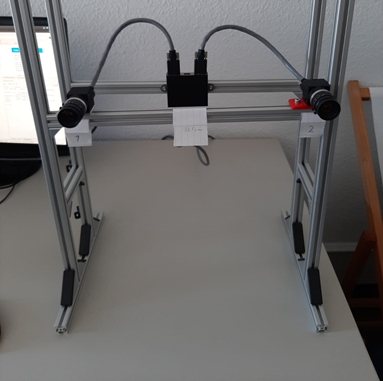
\includegraphics[scale=0.3]{bilder/camerasystem}
	\caption[Kamera-System]{Kamera-System}
\end{figure}

\noindent Mittels zwei Kameras, die auf einer Ebene angebracht sind (Stereonormalfall), kann der Mittelpunkt des Helikopters und dessen Abstand zur Kamera ermittelt werden.\newline
Zun"achst m"ussen daf"ur die Kameras einzeln und anschlie"send zu einander. Das Kalibrieren erfolgt "uber ein Schachbrett-Muster. Sind die Kameras zueinander kalibriert, kann mittels eines Feature-Detektors eine Punktewolke der Szene generiert und der Mittelpunkt des Helikopters berechnet werden.

\begin{figure}%
	\centering
	\subfloat[Kamera-Kalibrierung]{{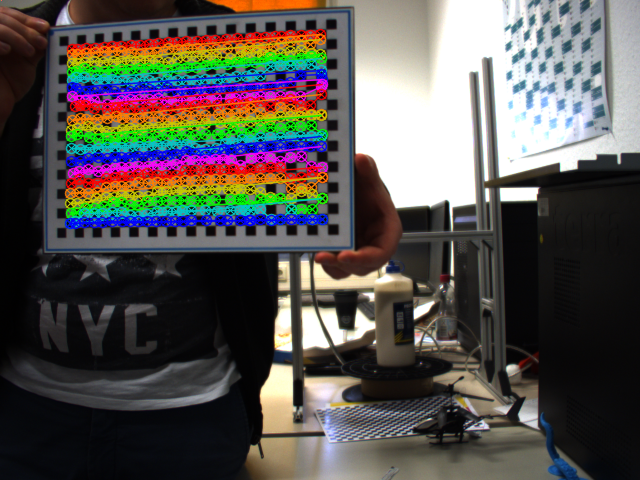
\includegraphics[width=6cm]{bilder/calibration} }}%
	\qquad
	\subfloat[Helikopter-Punktewolke mit berechneter Raumposition]{{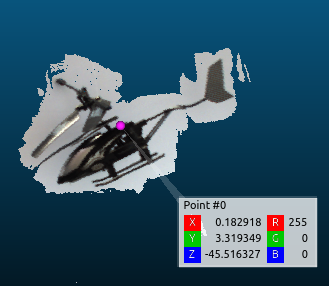
\includegraphics[width=6cm]{bilder/helicloud} }}%
	\caption{Kamera-Kalibrierung und Punktewolke}%
	\label{fig:extendetabstract}%
\end{figure}

